
\pdfminorversion=4 % for acroread
\documentclass[aspectratio=169,t,xcolor={usenames,dvipsnames}]{beamer}
%\documentclass[t,handout,xcolor={usenames,dvipsnames}]{beamer}
\usepackage{../beamerstyle}
\usepackage{dsfont}
\usepackage{bm}
\usepackage[english]{babel}
\usepackage[utf8]{inputenc}
\usepackage{graphicx}
\usepackage{algorithm}
\usepackage[ruled,vlined,algo2e,linesnumbered]{algorithm2e}
%\usepackage[boxed,vlined]{algorithm2e}
\usepackage{hyperref}
\usepackage{booktabs}
\usepackage{mathtools}

\usepackage{amsmath,amssymb}
\usepackage{listings}
\lstset{frame=lines,framesep=3pt,numbers=left,numberblanklines=false,basicstyle=\ttfamily\small}

\usepackage{subfig}
\usepackage{multicol}
%\usepackage{appendixnumberbeamer}
%
\usepackage{tcolorbox}

\usepackage{pgfplots}
\usepackage{tikz}
\usetikzlibrary{trees} 
\usetikzlibrary{shapes.geometric}
\usetikzlibrary{positioning,shapes,shadows,arrows,calc,mindmap}
\usetikzlibrary{positioning,fadings,through}
\usetikzlibrary{decorations.pathreplacing}
\usetikzlibrary{intersections}
\usetikzlibrary{positioning,fit,calc,shadows,backgrounds}
\pgfdeclarelayer{background}
\pgfdeclarelayer{foreground}
\pgfsetlayers{background,main,foreground}
\tikzstyle{activity}=[rectangle, draw=black, rounded corners, text centered, text width=8em]
\tikzstyle{data}=[rectangle, draw=black, text centered, text width=8em]
\tikzstyle{myarrow}=[->, thick, draw=black]

% Define the layers to draw the diagram
\pgfdeclarelayer{background}
\pgfdeclarelayer{foreground}
\pgfsetlayers{background,main,foreground}

%\usepackage{listings}
%\lstset{numbers=left,
%  showstringspaces=false,
%  frame={tb},
%  captionpos=b,
%  lineskip=0pt,
%  basicstyle=\ttfamily,
%%  extendedchars=true,
%  stepnumber=1,
%  numberstyle=\small,
%  xleftmargin=1em,
%  breaklines
%}

 
\definecolor{blue}{RGB}{0, 74, 153}

\usetheme{Boadilla}
%\useinnertheme{rectangles}
\usecolortheme{whale}
\setbeamercolor{alerted text}{fg=blue}
\useoutertheme{infolines}
\setbeamertemplate{navigation symbols}{\vspace{-5pt}} % to lower the logo
\setbeamercolor{date in head/foot}{bg=blue} % blue
\setbeamercolor{date in head/foot}{fg=white}
\setbeamercolor{author in head/foot}{bg=blue} %blue
\setbeamercolor{title in head/foot}{bg=blue} % blue
\setbeamercolor{title}{fg=white, bg=blue}
\setbeamercolor{block title}{fg=white,bg=blue}
\setbeamercolor{block body}{bg=blue!10}
\setbeamercolor{frametitle}{fg=white, bg=blue}
\setbeamercovered{invisible}

\makeatletter
\setbeamertemplate{footline}
{
  \leavevmode%
  \hbox{%
  \begin{beamercolorbox}[wd=.333333\paperwidth,ht=2.25ex,dp=1ex,center]{author in head/foot}%
    \usebeamerfont{author in head/foot}\insertshortauthor
  \end{beamercolorbox}%
  \begin{beamercolorbox}[wd=.333333\paperwidth,ht=2.25ex,dp=1ex,center]{title in head/foot}%
    \usebeamerfont{title in head/foot}\insertshorttitle
  \end{beamercolorbox}%
  \begin{beamercolorbox}[wd=.333333\paperwidth,ht=2.25ex,dp=1ex,right]{date in head/foot}%
    \usebeamerfont{date in head/foot}Week \@week, Topic \@topicnumber, Slide \insertframenumber{}\hspace*{2em}
%    \insertframenumber\hspace*{2ex} 
  \end{beamercolorbox}}%
  \vskip0pt%
}

\newcommand{\@week}{0}
\newcommand{\@topicnumber}{0}
\newcommand{\week}[1]{\renewcommand{\@week}{#1}}
\newcommand{\topicnumber}[1]{\renewcommand{\@topicnumber}{#1}}

\makeatother

%\pgfdeclareimage[height=1.2cm]{automl}{images/logos/automl.png}
%\pgfdeclareimage[height=1.2cm]{freiburg}{images/logos/freiburg}

%\logo{\pgfuseimage{freiburg}}

\input{../latex_main/macros}






\title[AutoML: Big Picture]{AutoML: Introduction}
\subtitle{The Big Picture}
\author[Marius Lindauer]{Bernd Bischl \and Frank Hutter \and Lars Kotthoff\newline \and \underline{Marius Lindauer} \and Joaquin Vanschoren}
\institute{}
\date{}
\week{1}
\topicnumber{1}



% \AtBeginSection[] % Do nothing for \section*
% {
%   \begin{frame}{Outline}
%     \bigskip
%     \vfill
%     \tableofcontents[currentsection]
%   \end{frame}
% }

\begin{document}
	
	\maketitle
	

%----------------------------------------------------------------------
%----------------------------------------------------------------------
%\begin{frame}[c]{In a Nutshell}

%\includegraphics[width=0.99\textwidth]{images/automl_comic}

%\end{frame}
%----------------------------------------------------------------------
%----------------------------------------------------------------------
\begin{frame}[c]{Machine Learning}

\centering
\textit{``Machine learning is the science of getting computers to act\\
 without being explicitly programmed.''}

\hfill by Andrew Ng

\end{frame}
%-----------------------------------------------------------------------
%----------------------------------------------------------------------
\begin{frame}[c]{Machine Learning requires many design decisions}

\centering
\includegraphics[width=0.8\textwidth]{images/sklearn-cheat}

\end{frame}
%-----------------------------------------------------------------------
%----------------------------------------------------------------------
\begin{frame}[c]{Machine Learning Workflow}

\centering
\input{tikz/ml-workflow}

\pause
 
\bigskip
\bigskip
\only<5->{$\leadsto$ Users indirectly teach machines how to learn.}

\end{frame}
%-----------------------------------------------------------------------
%----------------------------------------------------------------------
\begin{frame}[c]{Machine Learning does not scale up}

\begin{itemize}
  \item Basics in machine learning are not hard to grasp
  \smallskip
  \pause
  \item Achieving state-of-the-art performance is quite hard
  \smallskip
  \pause
  \item Design decisions are often not intuitive and\\ require a lot of expertise
  \begin{itemize}
    \item making these design decisions is a tedious and error-prone task
  \end{itemize}
 % \pause
  %\smallskip
%  \item Many experts are employed in ML these days
  \smallskip
  \pause
  \smallskip
  \item The job market for ML-experts is nearly empty
  \smallskip
  \pause
  \item Even with experts, developing new ML-applications takes time
\end{itemize}

\pause
\bigskip

Zoubin Ghahramani said that he often heard that:\\
\hfill \textit{``I'd like to use machine learning, but I can't invest much time.''}



\end{frame}
%-----------------------------------------------------------------------
%----------------------------------------------------------------------
%\begin{frame}[c]{AutoML Tools Demo}

%Auto-Sklearn:

%\url{https://colab.research.google.com/drive/11UcQQ_dymL5spF8o56qgSRZpMC1GKag9}

%\bigskip
%Auto-PyTorch:

%\url{https://colab.research.google.com/drive/14G5wvbqBkJ-SQJOdJsE_G8swq0JaFk6_}


%\end{frame}
%-----------------------------------------------------------------------
%----------------------------------------------------------------------
\begin{frame}[c]{Why does ML development take a lot of time?}

\centering
\includegraphics[width=1.0\textwidth]{images/MLPipeline.jpg}

\bigskip\bigskip\bigskip\bigskip
$\leadsto$ To achieve state-of-the-art performance,\\ this manual tuning has to be done for each new dataset again.

\end{frame}
%-----------------------------------------------------------------------
%----------------------------------------------------------------------
\begin{frame}[c]{A Simple Example with $k$-NN}

\centering
\includegraphics[width=0.5\textwidth]{images/kNN-jasmine}

\begin{itemize}
  \item $k$-nearest neighbors is one of the simplest ML algorithms
  \pause
  \item Size of neighbourhood ($k$) is very important for its performance
  \pause
  \item The performance function depending on $k$ is quite complex (not at all convex)
\end{itemize}

\end{frame}
%-----------------------------------------------------------------------
%----------------------------------------------------------------------
\begin{frame}[c]{Goal of AutoML}

\begin{block}{AutoML}
The goal of AutoML is to automate all parts of machine learning\\ (as needed)
to \emph{support} users efficiently building their ML-applications.
\end{block}

\bigskip
\pause

\begin{block}{Informal Definition: AutoML System}
Given
\begin{itemize}
  \item a dataset
  \item a task (e.g., regression or classification)
  \item a cost metric (e.g., accuracy or RMSE)
\end{itemize}
an AutoML system automatically determines the approach 
that performs best for this particular application.
\end{block}

\end{frame}
%-----------------------------------------------------------------------
%----------------------------------------------------------------------
\begin{frame}[c]{ML vs AutoML}

\begin{center}
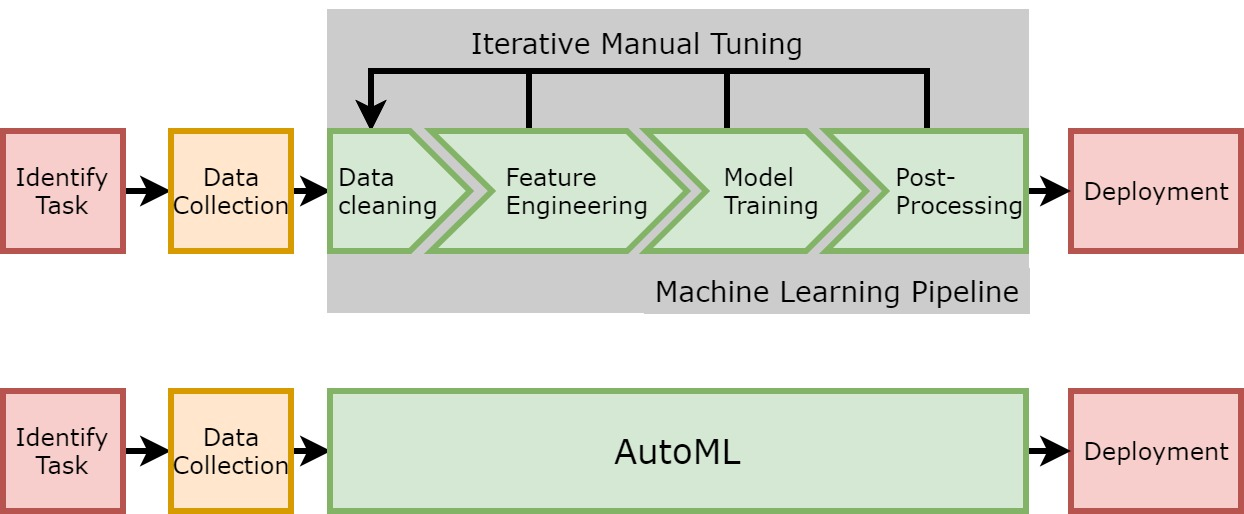
\includegraphics[width=0.7\textwidth]{images/AutoMLPipeline.jpg}
\end{center}

\bigskip
\pause
With AutoML, we ...
\begin{itemize}
	\item support ML users
	\item improve the efficiency of developping new ML applications
	\item reduce the required ML-expertise 
	\item might achieve better performance than developers w/o AutoML
\end{itemize}

\end{frame}
%-----------------------------------------------------------------------
%----------------------------------------------------------------------
\begin{frame}[c]{AutoML in Research}

AutoML enables:

\begin{enumerate}
  \item more efficient research
  \begin{itemize}
    \item AutoML has shown on subproblems to outperform human experts
  \end{itemize}
  \pause
  \smallskip
  \item more systematic research
  \begin{itemize}
    \item humans tend to be unsystematic which leads to errors
  \end{itemize}
  \smallskip
  \pause
  \item more reproducible research
  \begin{itemize}
    \item human's unsystematic approaches cannot be reproduced,\\ but AutoML is systematic
  \end{itemize}
  \smallskip
  \pause
  \item broader use of ML also in other disciplines
  \begin{itemize}
    \item ML should not be limited to computer scientists;
    \item the most amazing applications of ML are often done\\ by either interdisciplinary teams or even non-computer scientists
  \end{itemize}
\end{enumerate}

\end{frame}
%-----------------------------------------------------------------------
%----------------------------------------------------------------------
\begin{frame}[c]{Challenges in AutoML}

\begin{enumerate}
  \item Each dataset potentially require \alert{different optimal ML-designs}
  \begin{itemize}
    \item Design decisions have to be made for each dataset again
  \end{itemize}
  \smallskip
  \pause
  \item Training of a single ML model can be quite \alert{expensive}\\
  		(e.g., hours, days or weeks)
  \begin{itemize}
    \item often, we cannot try many design decisions
  \end{itemize}
  \smallskip
  \pause
  \item the \alert{mathematical relation} between design decisions\\ and performance is (often) \alert{unknown}
  \begin{itemize}
    \item gradient-based optimization is not directly possible
  \end{itemize}
  \smallskip
  \pause
  \item optimization in \alert{highly complex spaces}
  \begin{itemize}
    \item incl. categorical choices, continuous parameters,\\ conditional dependencies
  \end{itemize}
  
\end{enumerate}

\end{frame}
%-----------------------------------------------------------------------
%----------------------------------------------------------------------
%\begin{frame}[c]{Snippet of Auto-AI Hierarchy}

%\centering
%\includegraphics[width=0.5\textwidth]{images/autoai}

%\end{frame}
%-----------------------------------------------------------------------
\end{document}
